\documentclass[12pt,letterpaper]{exam}
\usepackage[lmargin=1in,rmargin=1in,tmargin=1in,bmargin=1in]{geometry}
\usepackage{../style/exams}

% -------------------
% Course & Exam Information
% -------------------
\newcommand{\course}{MAT 307: Exam 2}
\newcommand{\term}{Spring -- 2023}
\newcommand{\examdate}{04/17/2023}
\newcommand{\timelimit}{85 Minutes}

\setbool{hideans}{true} % Student: True; Instructor: False

% -------------------
% Content
% -------------------
\begin{document}

\examtitle
\instructions{Write your name on the appropriate line on the exam cover sheet. This exam contains \numpages\ pages (including this cover page) and \numquestions\ questions. Check that you have every page of the exam. Indicate your answer for each question in the answer column in the table below. You need not indicate your answers for each question both on the cover page and in the subsequent pages. You may show as much or as little work as you would like; however, only the answers on this cover page will be graded. Be sure each answer is legible and in the correct box. Do not write in the `Points' box on this page.} 
%\scores
%\bottomline

\vfill

\begin{table}[!ht]
\centering
\begin{tabular}{|
>{\columncolor[HTML]{C0C0C0}}c |c|
>{\columncolor[HTML]{C0C0C0}}c |c|
>{\columncolor[HTML]{C0C0C0}}c |c|}
\hline
\cellcolor[HTML]{000000}{\color[HTML]{FFFFFF} \textbf{Question}} & \cellcolor[HTML]{000000}{\color[HTML]{FFFFFF} \textbf{Answer}} & \cellcolor[HTML]{000000}{\color[HTML]{FFFFFF} \textbf{Question}} & \cellcolor[HTML]{000000}{\color[HTML]{FFFFFF} \textbf{Answer}} & \cellcolor[HTML]{000000}{\color[HTML]{FFFFFF} \textbf{Question}} & \cellcolor[HTML]{000000}{\color[HTML]{FFFFFF} \textbf{Answer}} \\ \hline
1 &  & 11 &  & 21 &  \\ \hline
2 &  & 12 &  & 22 &  \\ \hline
3 &  & 13 &  & 23 &  \\ \hline
4 &  & 14 &  & 24 &  \\ \hline
5 &  & 15 &  & 25 &  \\ \hline
6 &  & 16 &  & 26 &  \\ \hline
7 &  & 17 &  & 27 &  \\ \hline
8 &  & 18 &  & 28 &  \\ \hline
9 &  & 19 &  & 29 &  \\ \hline
10 &  & 20 &  & 30 &  \\ \hline
\end{tabular}
\end{table}

\vspace{0.5cm}

	\begin{table}[!ht]
	\centering
	\begin{tabular}{|c|c|} \hline 
	\rowcolor[HTML]{000000} 
	{\color[HTML]{FFFFFF} Points} & {\color[HTML]{FFFFFF} Total} \\ \hline
	& 30 \\ \hline
	\end{tabular}
	\end{table}

\vspace{3cm}
\vfill

\newpage


% ---------
% Questions
% ---------
\begin{questions}

% Question 1 - a
\question If lines $\ell_1$ and $\ell_2$ are parallel and $\ell_3$ is not parallel to $\ell_1$, which of the following is true. 
	\begin{enumerate}[A.]
	\item $\ell_3$ is parallel to $\ell_2$. % Correct
	\item $\ell_3$ intersects $\ell_2$.
	\item $\ell_3$ is concurrent to $\ell_1$ and $\ell_2$.
	\item $\ell_3$ cannot be a transversal to $\ell_1$ and $\ell_2$. 
	\end{enumerate}



\vfill



% Question 2 - c
\question What is the value of the angle $x$ in the triangle below?
	\[
	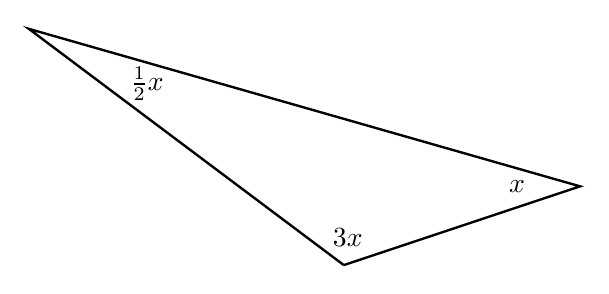
\begin{tikzpicture}
	\draw[line width=0.03cm] (0,0) -- (3,1) -- (-4,3) -- (0,0);
	\node at (-2.5,2.3) {$\frac{1}{2}x$};
	\node at (0.05,0.35) {$3x$};
	\node at (2.2,1) {$x$};
	\end{tikzpicture}
	\]

\begin{enumerate}[A.]
\item $30^\circ$
\item $40^\circ$
\item $80^\circ$ % Correct
\item $120^\circ$
\end{enumerate}



\vfill



% Question 3 - b
\question How many degrees does the hour hand of a clock move in 40 minutes?
        \begin{enumerate}[A.]
        \item $20^\circ$
        \item $30^\circ$ % Correct
        \item $40^\circ$
        \item $240^\circ$
        \end{enumerate}



\vfill



% Question 4 - b
\question What angle is formed using the minute and hour hand of a clock at 4:30?
        \begin{enumerate}[A.]
        \item $30^\circ$
        \item $45^\circ$ % Correct
        \item $120^\circ$
        \item $135^\circ$
        \end{enumerate}



\newpage



% Question 5 - d
\question When measured from the positive $x$-axis (the initial side), which of the following angle has the same as terminal side as the angle $120^\circ$?
        \begin{enumerate}[A.]
        \item $-240^\circ$
        \item $-60^\circ$
        \item $60^\circ$
        \item $240^\circ$ % Correct
        \end{enumerate}



\vfill



% Question 6 - b
\question If the triangle below has whole number angles and is drawn to scale, which of the following is the largest possible measure for the angle $\theta$?
	\[
	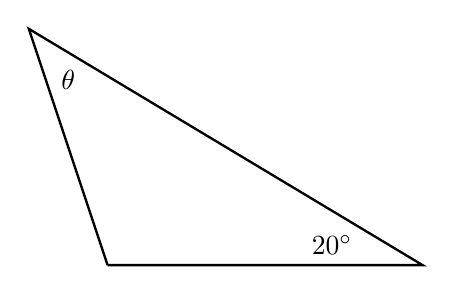
\begin{tikzpicture}
	\draw[line width=0.03cm] (0,0) -- (4,0) -- (-1,3) -- (0,0);
	\node at (-0.5,2.35) {$\theta$};
	\node at (2.85,0.25) {$20^\circ$};
	\end{tikzpicture}
	\]

\begin{enumerate}[A.]
\item $20^\circ$
\item $69^\circ$ % Correct
\item $70^\circ$
\item $90^\circ$
\end{enumerate}



\vfill



% Question 7 - c
\question Which of the following angles is vertical to angle $\theta$ in the diagram below?
	\[
	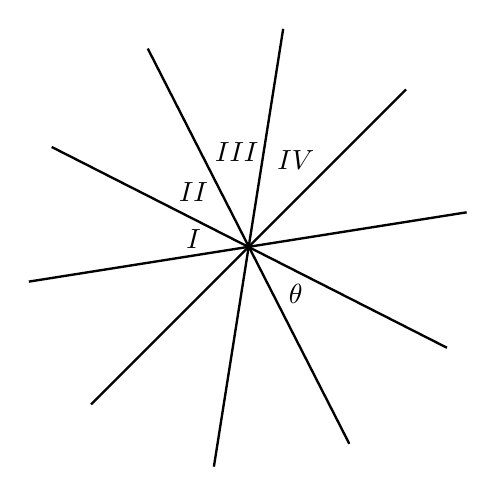
\begin{tikzpicture}
	\draw[line width=0.03cm] (-2,-2) -- (2,2);
	\draw[line width=0.03cm] (1.28,-2.5) -- (-1.28, 2.52);
	\draw[line width=0.03cm] (2.77,0.44) -- (-2.79,-0.44);
	\draw[line width=0.03cm] (0.44,2.77) -- (-0.44,-2.79);
	\draw[line width=0.03cm] (-2.50,1.27) -- (2.52,-1.28);
	\node at (0.6,-0.6) {$\theta$};
	\node at (-0.7,0.1) {$I$};
	\node at (-0.7,0.7) {$II$};
	\node at (-0.15,1.2) {$III$};
	\node at (0.6,1.1) {$IV$};
	\end{tikzpicture}
	\]
	
\begin{enumerate}[A.]
\item $I$
\item $II$
\item $III$ % Correct
\item $IV$
\end{enumerate}



\newpage



% Question 8 - a
\question What is the measure of the angle $\theta$ in the triangle below?
	\[
	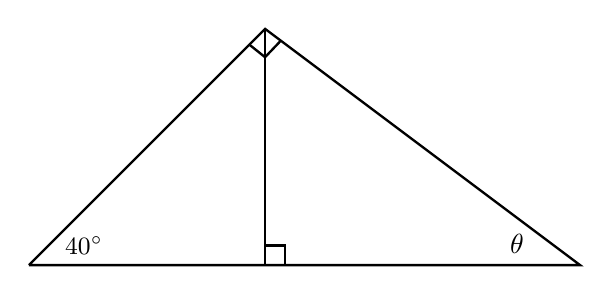
\begin{tikzpicture}
	\draw[line width=0.03cm] (-3,0) -- (4,0) -- (0,3) -- (-3,0);
	\draw[line width=0.03cm] (0,3) -- (0,0);
	\draw[line width=0.03cm] (0,0.25) -- (0.25,0.25) -- (0.25,0);
	\draw[line width=0.03cm] (-0.2,2.8) -- (0,2.64) -- (0.2,2.85);
	\node at (-2.3,0.25) {\small$40^\circ$};
	\node at (3.2,0.27) {$\theta$};
	\end{tikzpicture}
	\]

\begin{enumerate}[A.]
\item $40^\circ$ % Correct
\item $45^\circ$
\item $50^\circ$
\item $60^\circ$
\end{enumerate}



\vfill




% Question 9 - c
\question What is the measure of angle $f$ in the diagram below?
	\[
	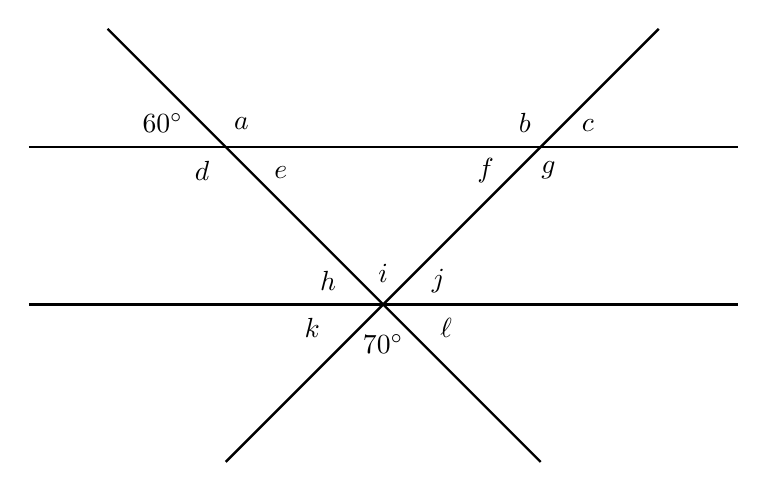
\begin{tikzpicture}
	\draw[line width=0.03cm] (-4.5,2) -- (4.5,2);
	\draw[line width=0.03cm] (-4.5,0) -- (4.5,0);
	\draw[line width=0.03cm] (-2,-2) -- (3.5,3.5);
	\draw[line width=0.03cm] (-3.5,3.5) -- (2,-2);
	\node at (-2.8,2.3) {$60^\circ$};
	\node at (-1.8,2.3) {$a$};
	\node at (1.8,2.3) {$b$};
	\node at (2.6,2.27) {$c$};
	\node at (-2.3,1.7) {$d$};
	\node at (-1.3,1.67) {$e$};
	\node at (1.3,1.7) {$f$};
	\node at (2.1,1.7) {$g$};
	\node at (-0.7,0.3) {$h$};
	\node at (0,0.4) {$i$};
	\node at (0.7,0.3) {$j$};
	\node at (-0.9,-0.3) {$k$};
	\node at (0,-0.5) {$70^\circ$};
	\node at (0.8,-0.3) {$\ell$};
	\end{tikzpicture}
	\]

\begin{enumerate}[A.]
\item $40^\circ$
\item $50^\circ$
\item $60^\circ$ % Correct
\item $70^\circ$
\end{enumerate}



\vfill



% Question 10 - c
\question Which of the following {\itshape does not} force two lines cut by a transversal to be parallel?
        \begin{enumerate}[A.]
        \item The alternate interior angles are congruent. 
        \item The corresponding angles are congruent. 
        \item The vertical angles are congruent. % Correct
        \item The alternate exterior angles are congruent. 
        \end{enumerate}



\newpage



% Question 11 - b
\question Which of the following best describes the curve shown below?
	\[
	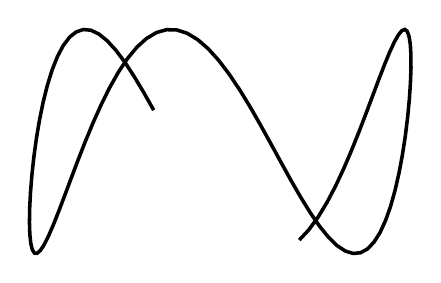
\begin{tikzpicture}[scale=3]
	\begin{axis}[
	xmin=-8,xmax=4,
	ymin=-8,ymax=4,
	grid=none,
	axis lines=none
	]
	\addplot[line width=0.015cm, domain= -2:3.5,samples=100] ({sin(deg(x)) - cos(deg(x))}, {sin(3*deg(x))});
	\end{axis}
	\end{tikzpicture}
	\]

\begin{enumerate}[A.]
\item A simple curve.
\item A closed curve. % Correct
\item A simple, closed curve. 
\item A non-simple, curve. 
\end{enumerate}



\vfill



% Question 12 - a
\question How many convex figures are shown below?
	\[
	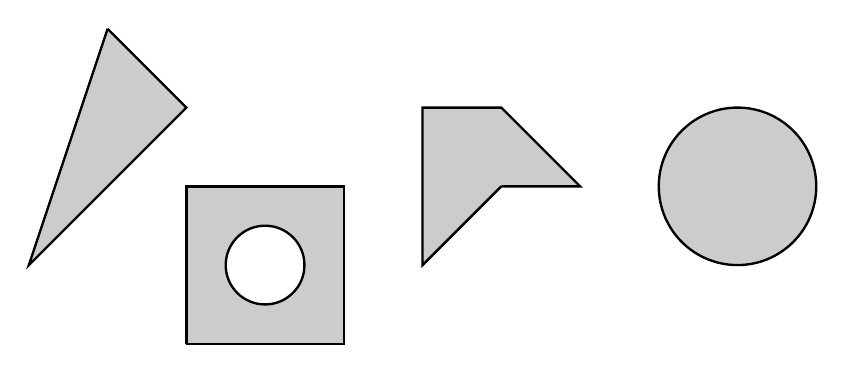
\begin{tikzpicture}
	\draw[line width=0.03cm,fill=gray!40] (3,3) circle (1);
	\draw[line width=0.03cm,fill=gray!40] (-5,5) -- (-4,4) -- (-6,2) -- (-5,5);
	\draw[line width=0.03cm,fill=gray!40] (0,3) -- (-1,2) -- (-1,4) -- (0,4) -- (1,3) -- (0,3);
	\draw[line width=0.03cm,fill=gray!40] (-4,1) -- (-4,3) -- (-2,3) -- (-2,1) -- (-4,1);
	\draw[line width=0.03cm,fill=white] (-3,2) circle (0.5);
	\end{tikzpicture}
	\]

\begin{enumerate}[A.]
\item 1 % Correct
\item 2
\item 3
\item 4
\end{enumerate}



\vfill



% Question 13 - d
\question Which of the following cannot be the sum of the interior angles of a convex $n$-gon?
        \begin{enumerate}[A.]
        \item $180^\circ$
        \item $360^\circ$
        \item $1260^\circ$
        \item $2250^\circ$ % Correct
        \end{enumerate}



\newpage



% Question 14  - b
\question Which of the following cannot be the measure of an interior angle of a regular polygon?
        \begin{enumerate}[A.]
        \item $60^\circ$
        \item $90^\circ$ % Correct
        \item $158^\circ$
        \item $168^\circ$
        \end{enumerate}



\vfill



% Question 15 - c
\question Find the total turn for the closed curve shown below if one traverses the curve clockwise. 
	\[
	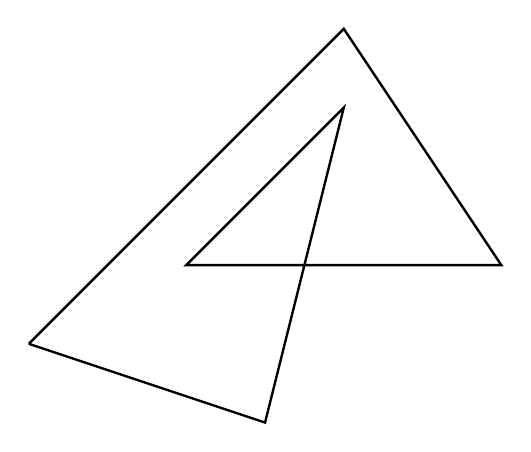
\begin{tikzpicture}
	\draw[line width=0.03cm] (-1,0) -- (2,-1) -- (3,3) -- (1,1) -- (5,1) -- (3,4) -- (-1,0);
	\end{tikzpicture}
	\]

\begin{enumerate}[A.]
\item $-720^\circ$
\item $-360^\circ$
\item $0^\circ$ % Correct
\item $360^\circ$
\end{enumerate}



\vfill



% Question 16 - d
\question Which of the following statements is \textit{true}?
        \begin{enumerate}[A.]
        \item All rectangles are rhombuses.
        \item All rhombuses are rectangles.
        \item Some rhombuses are rectangles.
        \item There are no rectangles that are rhombuses. % Correct
        \end{enumerate}



\vfill



% Question 17 - c
\question Which of the following statements is \textit{false}?
        \begin{enumerate}[A.]
        \item Rectangles are isosceles trapezoids. 
        \item There are no squares that are not also a rhombus. 
        \item Triangles are never parallelograms. % Correct
        \item A trapezoid can never be a parallelogram. 
        \end{enumerate}



\newpage



% Question 18 - a
\question A convex, five-sided polygon has angles $110^\circ$, $90^\circ$, $120^\circ$, and $100^\circ$. Find the measure of the missing angle. 
%	\[
%	\begin{tikzpicture}[scale=1.3]
%	\draw[line width=0.03cm] (1.3050,0) -- (1,-0.9511) -- (0,-0.9511) -- (0.8050,-1.5388) -- (0.5,-2.4899) -- (1.3050,-1.9021) -- (2.1180,-2.4899) -- (1.8090,-1.5388) -- (2.6180,-0.9511) -- (1.6180,-0.9511) -- (1.3050,0);
%	\end{tikzpicture}
%	\]

        \begin{enumerate}[A.]
        \item $90^\circ$ % Correct
        \item $100^\circ$
        \item $120^\circ$
        \item $160^\circ$
        \end{enumerate}



\vfill



% Question 19 - d
\question Which of the following is \textit{true}?
        \begin{enumerate}[A.]
        \item The total turn around any polygon is $360^\circ$.
        \item All $n$-gons have interior angles whose sum is $(n - 2)180^\circ$.
        \item The sum of the exterior angles to a nonagon is $1260^\circ$.
        \item A general polygon can have sides which intersect at a point other than their endpoints. % Correct
        \end{enumerate}



\vfill



% Question 20 - c
\question What is the measure of the interior angles of a regular octagon?
        \begin{enumerate}[A.]
        \item $45^\circ$
        \item $135^\circ$
        \item $1080^\circ$ % Correct
        \item $1440^\circ$
        \end{enumerate}



\vfill



% Question 21 - a
\question Which of the following statements is \textit{true}. 
        \begin{enumerate}[A.]
        \item The interior angles of a regular $n$-gon are always greater than their exterior angles. % Correct
        \item The exterior angles of a regular $n$-gon are always greater than their interior angles.
        \item The interior angles of a regular $n$-gon are almost always greater than their exterior angles.
        \item The interior and exterior angles of a regular $n$-gon are never congruent. 
        \end{enumerate}



\vfill



% Question 22 - c
\question Which of the following are sometimes a regular $n$-gon?
        \begin{enumerate}[A.]
        \item A circle.
        \item A rectangle. 
        \item A figure eight. % Correct
        \item A non-isosceles trapezoid. 
        \end{enumerate}



\newpage



% Question 23 - a
\question Aleksandr is reading about US History. He reads that George Washington only made \$2.50 every fortnight. How much is this in euro per week? [1 fortnight $=$ 2 weeks; \par \texteuro 1 $=$ \$1.10]
        \begin{enumerate}[A.]
        \item \texteuro 1.14 per week % Correct
        \item \texteuro 1.38 per week
        \item \texteuro 2.55 per week
        \item \texteuro 4.54 per week 
        \end{enumerate}



\vfill



% Question 24 - a
\question A large circular room is 15~ft across. What is the area of this room in square inches?
        \begin{enumerate}[A.]
        \item 58.9~in$^2$ % Correct
        \item 706.9~in$^2$
        \item 2,120.6~in$^2$
        \item 25,446.9~in$^2$
        \end{enumerate}



\vfill



% Question 25 - c
\question Find $s$ in the diagram below:
	\[
	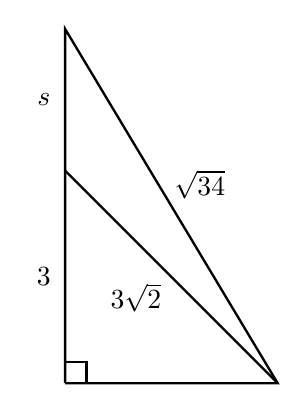
\begin{tikzpicture}[scale=0.9]
	\draw[line width=0.03cm] (0,0) -- (0,5) -- (3,0) -- (0,0);
	\draw[line width=0.03cm] (0,0.3) -- (0.3,0.3) -- (0.3,0);
	\draw[line width=0.03cm] (3,0) -- (0,3);
	\node at (-0.3,1.5) {$3$};
	\node at (1.9,2.8) {$\sqrt{34}$};
	\node at (1,1.2) {$3\sqrt{2}$};
	\node at (-0.3,4.0) {$s$};
	\end{tikzpicture}
	\]

\begin{enumerate}[A.]
\item $2$
\item $3$
\item $8$ % Correct
\item $12$
\end{enumerate}



\vfill



% Question 26 - b
\question What is the volume of a can of soda if the can is approximately a right circular cylinder with height 4.8~in and is 2.6~in across?
        \begin{enumerate}[A.]
        \item $19.6$~in$^3$
        \item $25.5$~in$^3$ % Correct
        \item $39.2$~in$^3$
        \item $123.2$~in$^3$
        \end{enumerate}



\newpage



% Question 27 - c
\question You are wrapping a large holiday gift for a friend. The box is oddly (but regularly shaped) at the base but you estimate the base has area $7.34$~ft$^2$ and perimeter $15.5$~ft. The box narrows to a point at the top and is generally shaped like a pyramid. The slanted height of the entire box is $3.5$~ft. What is approximately the least amount of wrapping paper it will take to cover the gift?
        \begin{enumerate}[A.]
        \item $34.5$~ft$^3$
        \item $41.2$~ft$^3$
        \item $96.2$~ft$^3$ % Correct
        \item $398.2$~ft$^3$
        \end{enumerate}



\vfill



% Question 28 - d
\question You want to paint a small wood working box that you made. The box has a rectangular base that measure 1.5~ft by 3.6~ft. The box is open at the top and is 0.75~ft tall. What is the surface area of the box?
        \begin{enumerate}[A.]
        \item $4.05$~ft$^2$
        \item $5.85$~ft$^2$
        \item $13.05$~ft$^2$
        \item $18.45$~ft$^2$ % Correct
        \end{enumerate}



\vfill



% Question 29 - b
\question What is the volume of a cone that is 10~cm tall and whose base is a circle that measures 5~cm across?
        \begin{enumerate}[A.]
        \item $52.4$~cm$^3$
        \item $65.4$~cm$^3$ % Correct
        \item $261.8$~cm$^3$
        \item $785.4$~cm$^3$
        \end{enumerate}



\vfill



% Question 30 - a
\question What is the area of the region shaded below?
	\[
	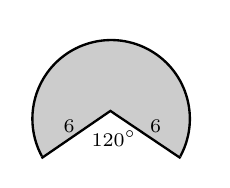
\begin{tikzpicture}
	\draw[line width=0.03cm,fill=gray!40] (0,0) arc (-30:210:1);
	\draw[line width=0.03cm,fill=white,white] (-1.75,0) -- (-0.875,0.6) -- (0.017,0) -- (-1.75,0);
	\draw[line width=0.03cm] (-1.75,0) -- (-0.875,0.6) -- (0.017,0);
	\node at (-0.3,0.4) {\scriptsize$6$};
	\node at (-1.4,0.4) {\scriptsize$6$};
	\node at (-0.83,0.25) {\scriptsize$120^\circ$};
	\end{tikzpicture}
	\]

\begin{enumerate}[A.]
\item $0.94$ % Correct
\item $75.4$
\item $37.7$
\item $233.1$
\end{enumerate}


\end{questions}
\end{document}